%%%%% METHNAME %%%%%%%%%%%%%%%%%%%%%%%%%%
\begin{figure}[h]
  \centering
    \subfigure[]{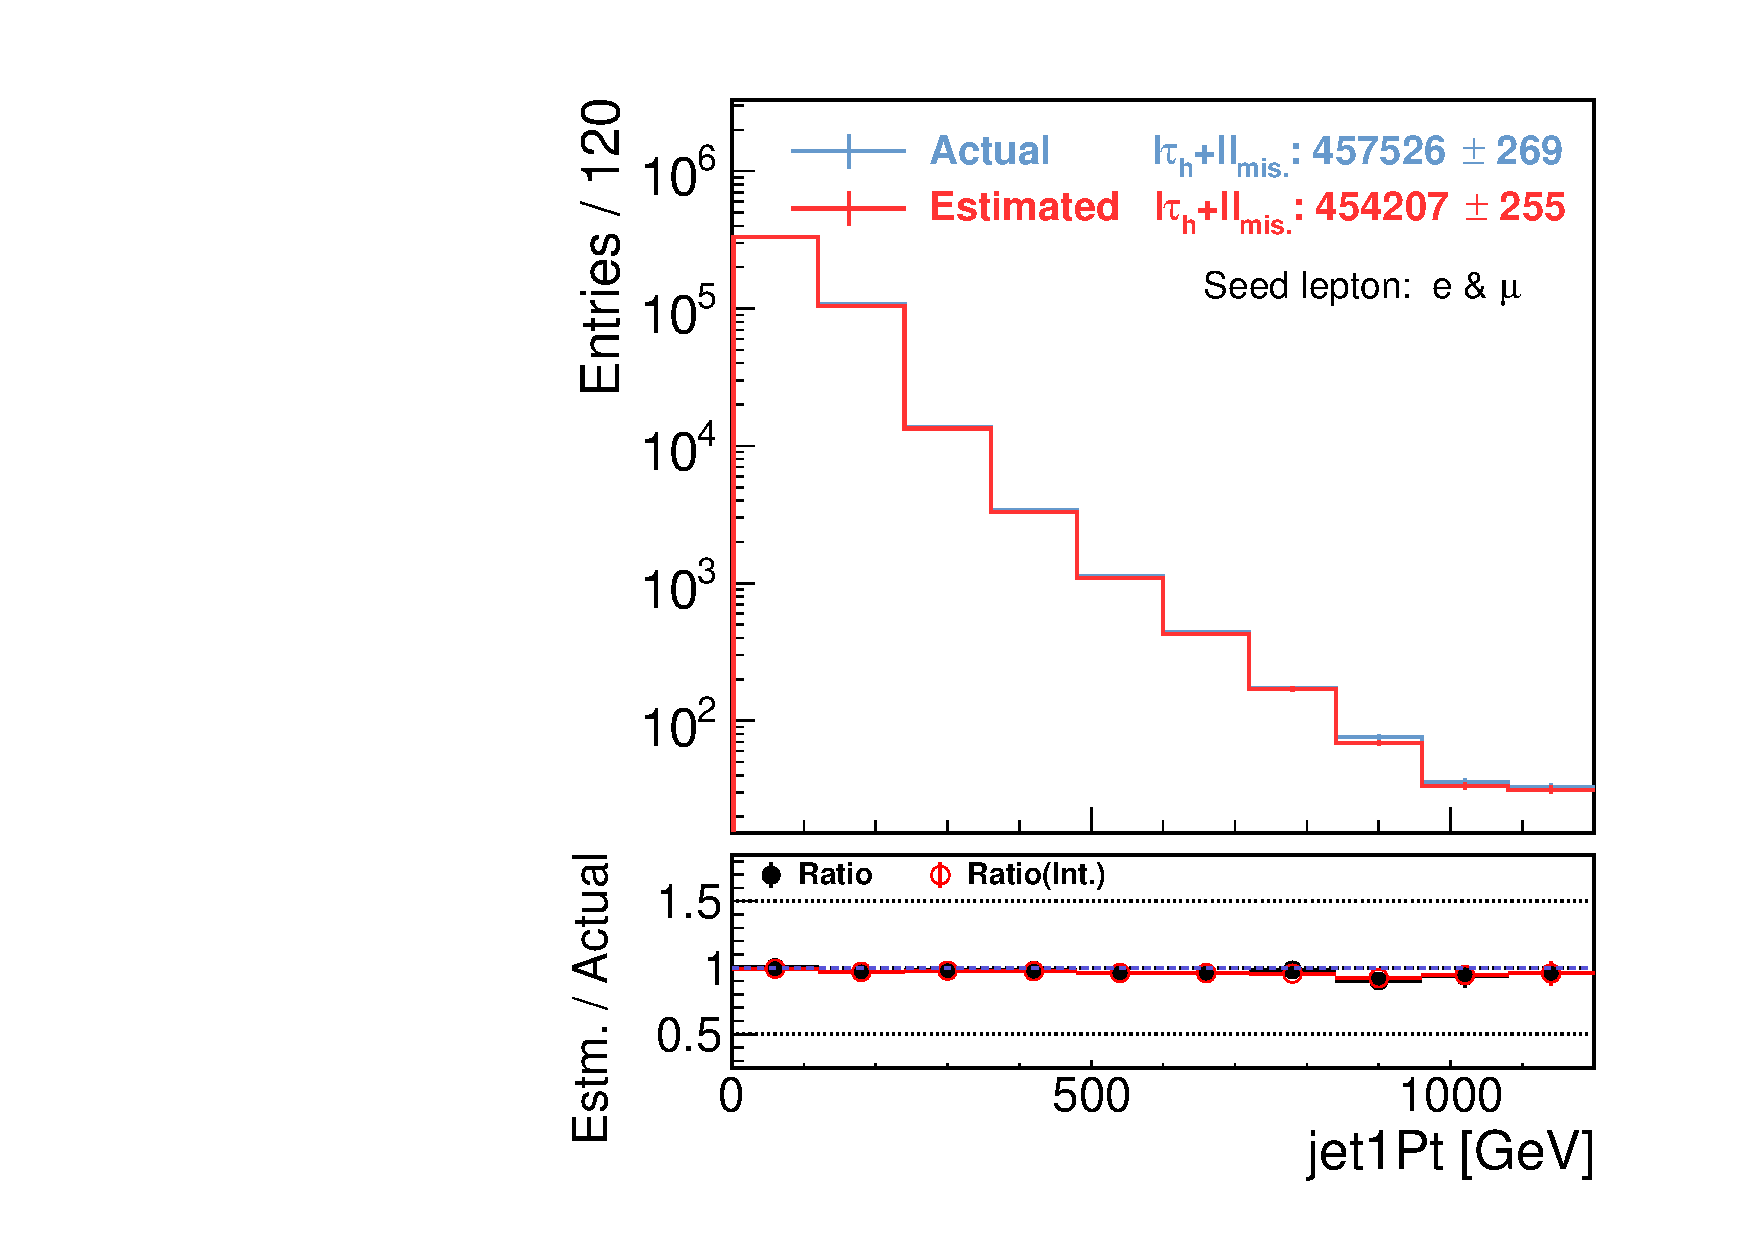
\includegraphics[width=0.32\textwidth]{figures/BGestimation/ObjReplacement/mcClosure/All_emu/All_emu_jet1Pt__trMode4_NoSys.pdf}}
    \subfigure[]{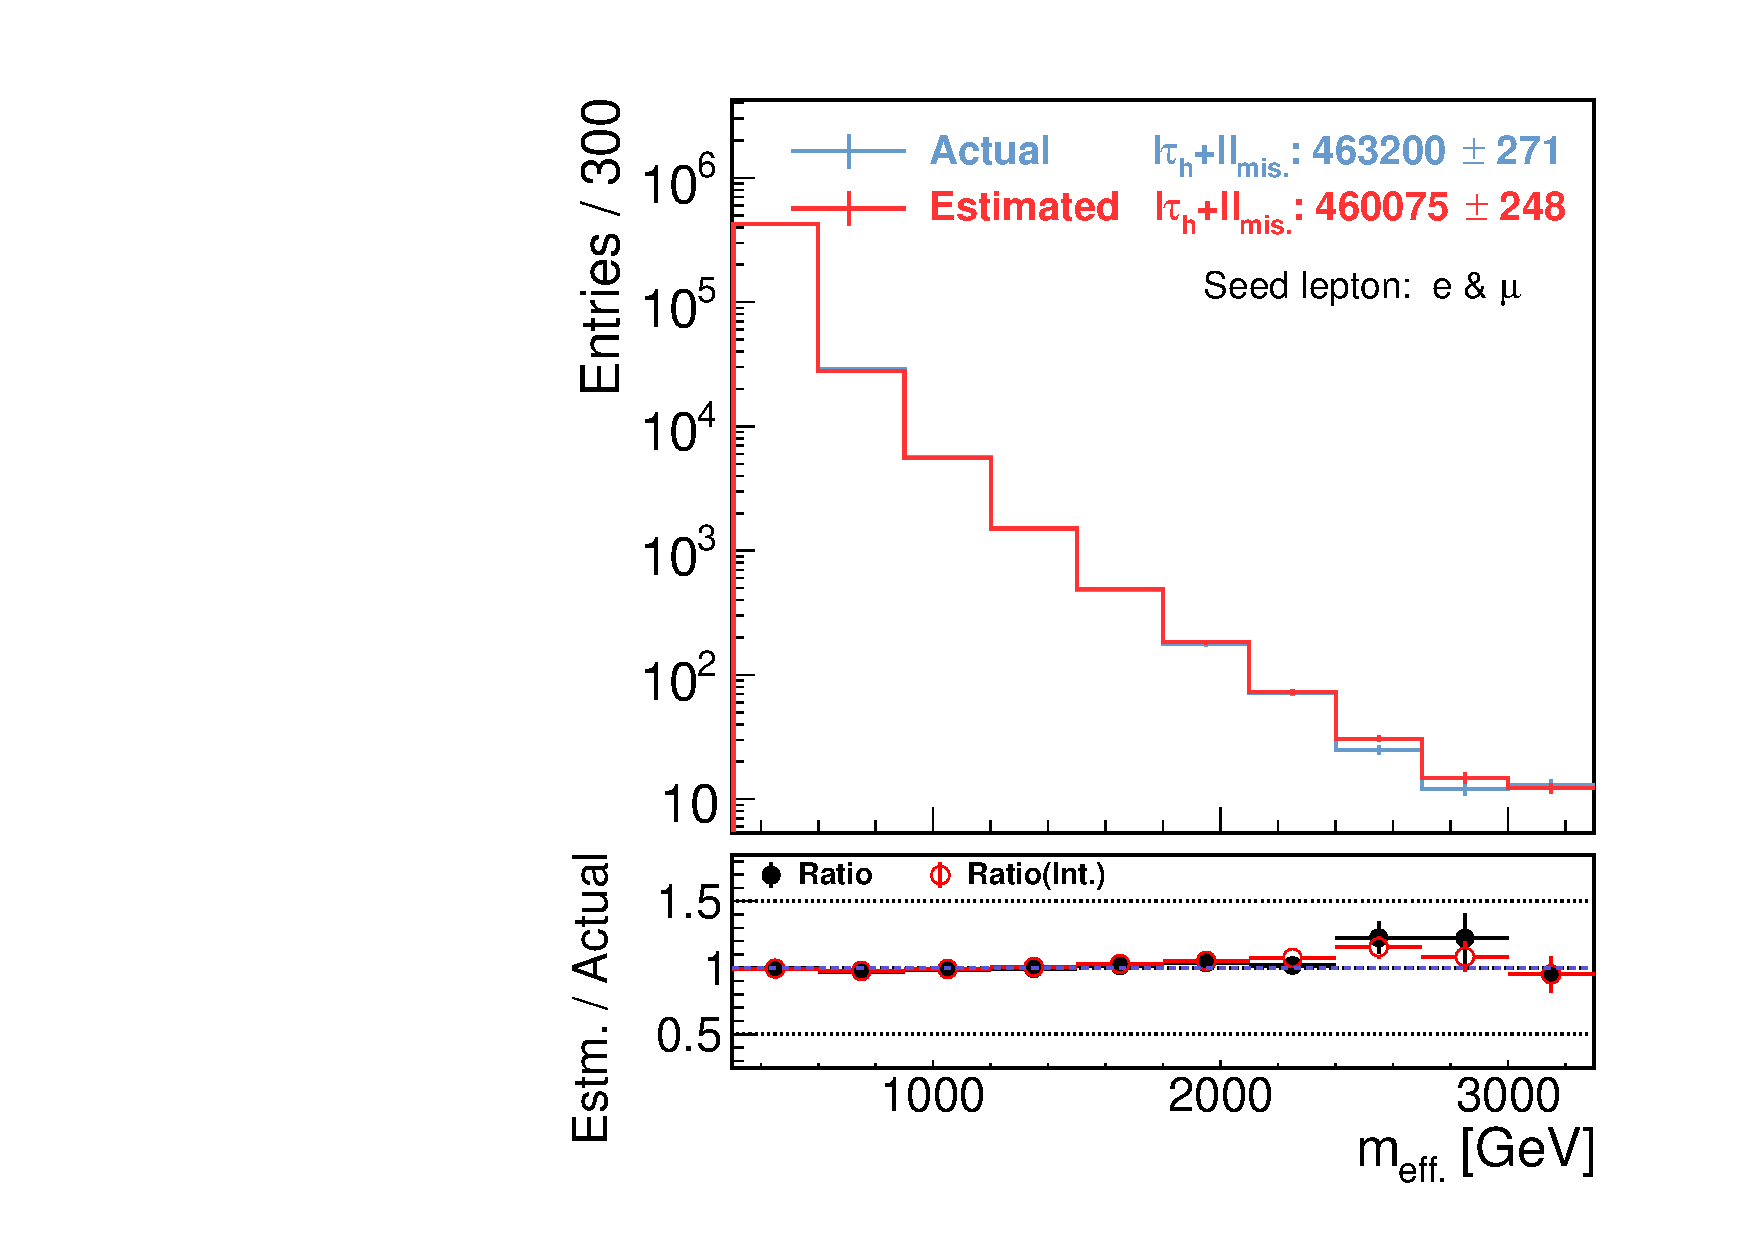
\includegraphics[width=0.32\textwidth]{figures/BGestimation/ObjReplacement/mcClosure/All_emu/All_emu_meffInc30__trMode4_NoSys.pdf}}
    \subfigure[]{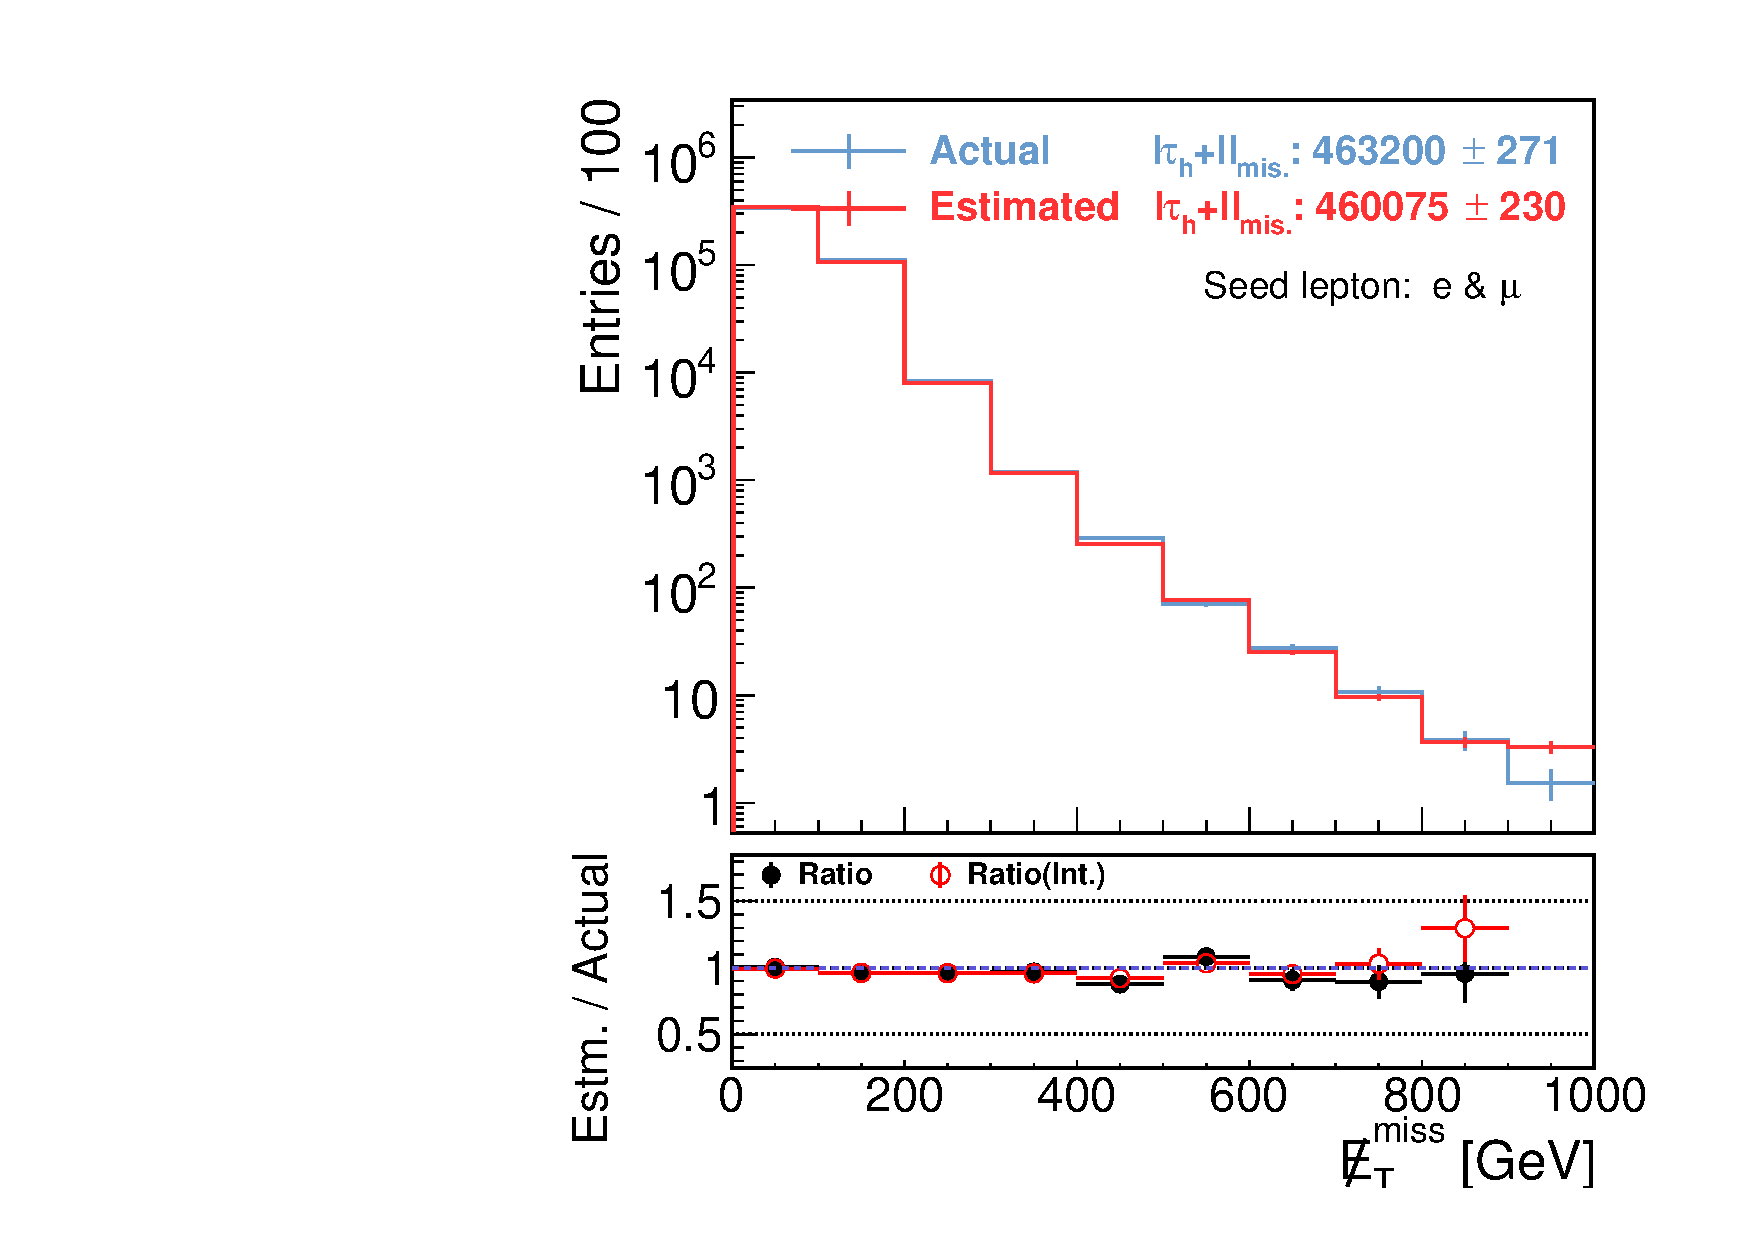
\includegraphics[width=0.32\textwidth]{figures/BGestimation/ObjReplacement/mcClosure/All_emu/All_emu_met__trMode4_NoSys.pdf}}
    \subfigure[]{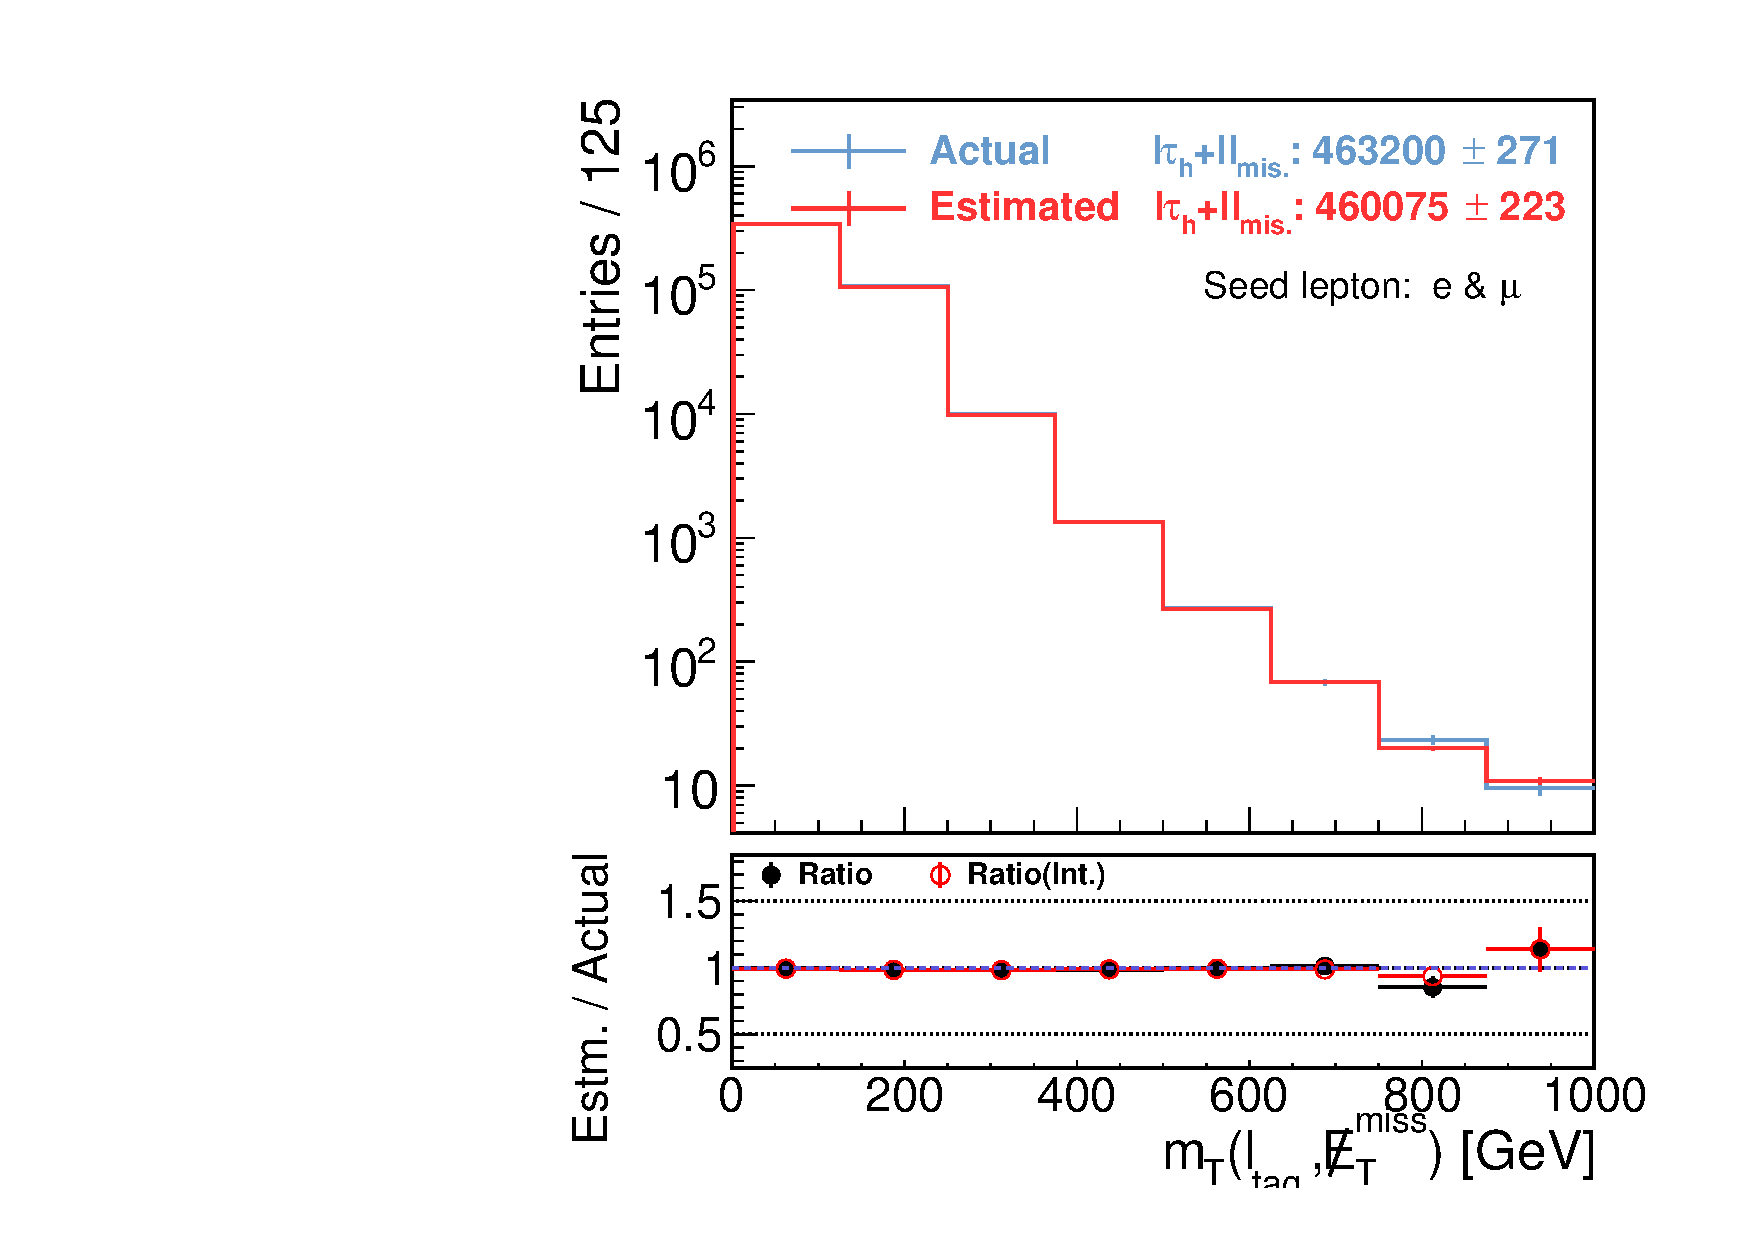
\includegraphics[width=0.32\textwidth]{figures/BGestimation/ObjReplacement/mcClosure/All_emu/All_emu_mt__trMode4_NoSys.pdf}}
    \subfigure[]{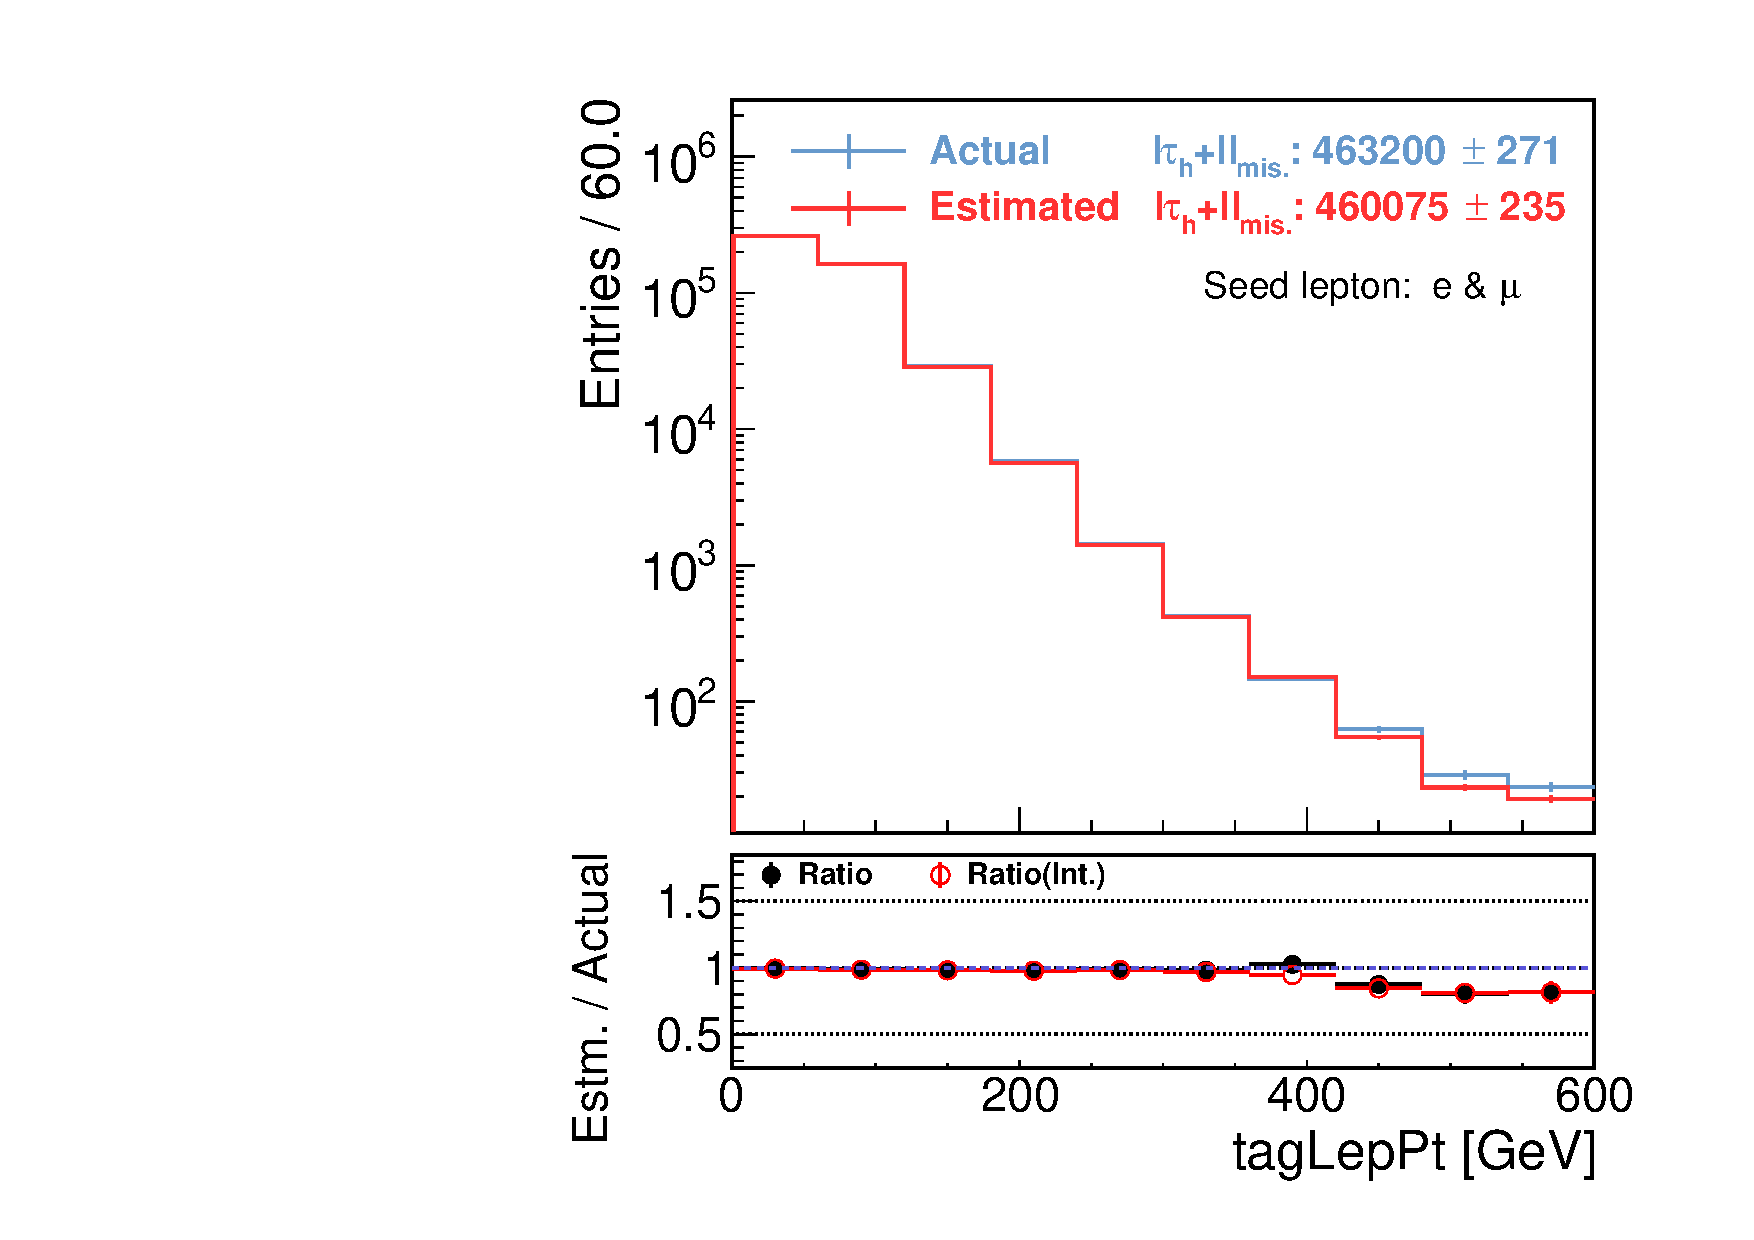
\includegraphics[width=0.32\textwidth]{figures/BGestimation/ObjReplacement/mcClosure/All_emu/All_emu_tagLepPt__trMode4_NoSys.pdf}}
    \subfigure[]{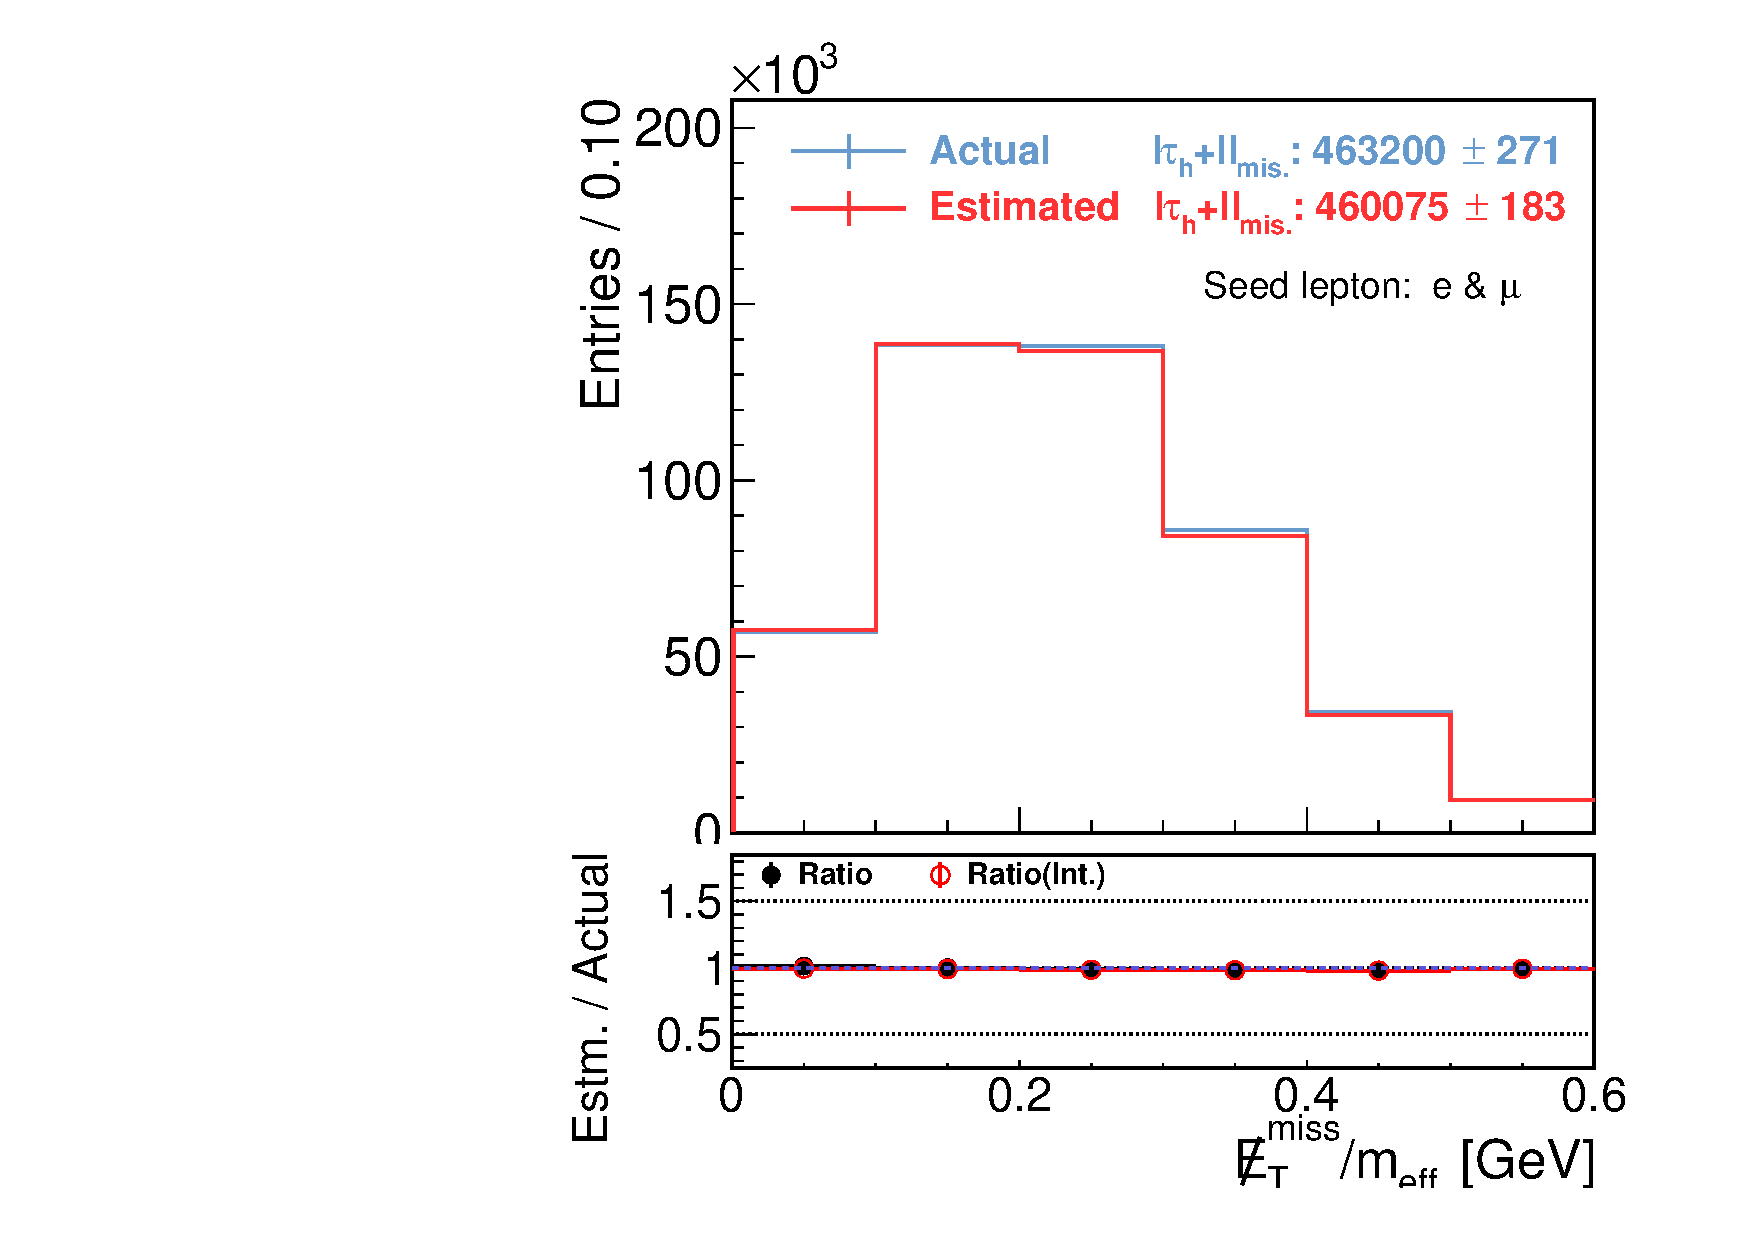
\includegraphics[width=0.32\textwidth]{figures/BGestimation/ObjReplacement/mcClosure/All_emu/All_emu_metOverMeff__trMode4_NoSys.pdf}}
    \subfigure[]{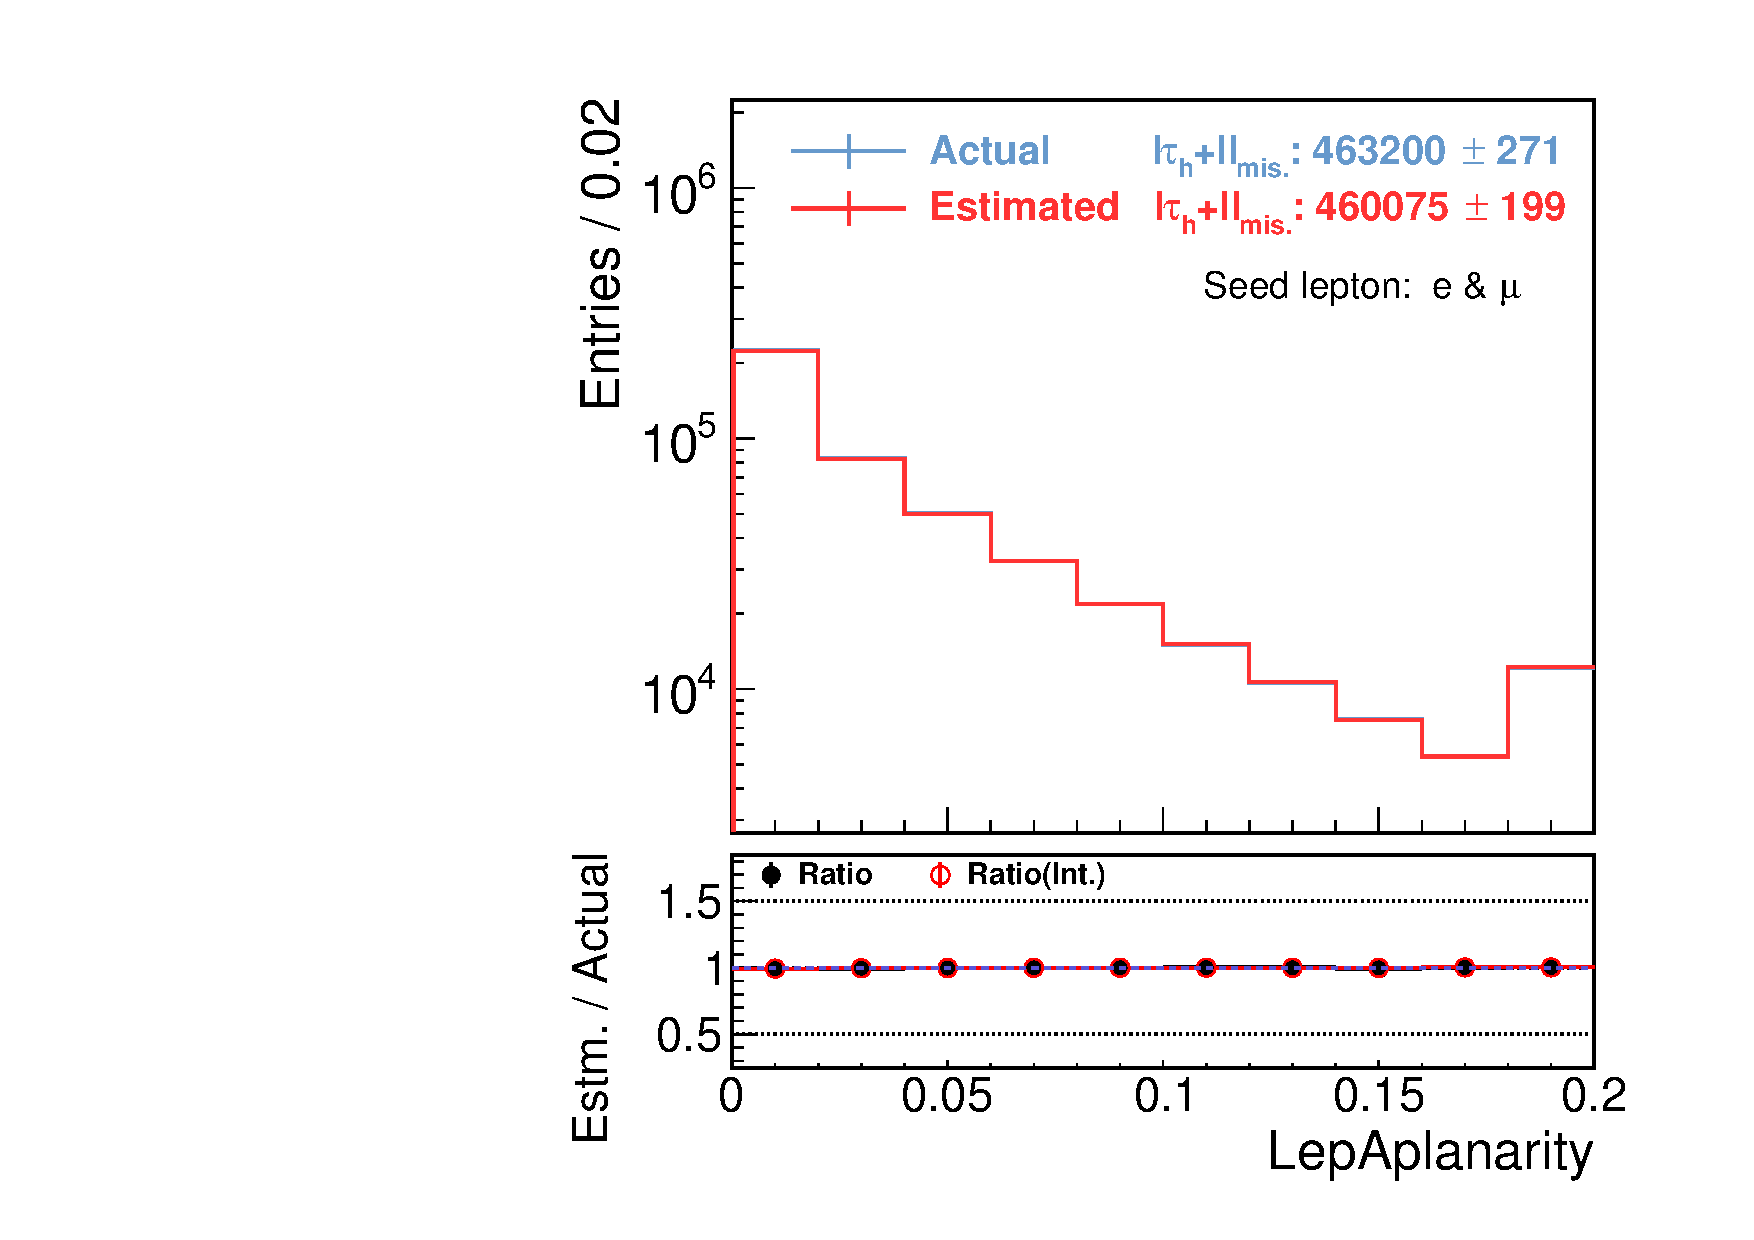
\includegraphics[width=0.32\textwidth]{figures/BGestimation/ObjReplacement/mcClosure/All_emu/All_emu_LepAplanarity__trMode4_NoSys.pdf}}
    \subfigure[]{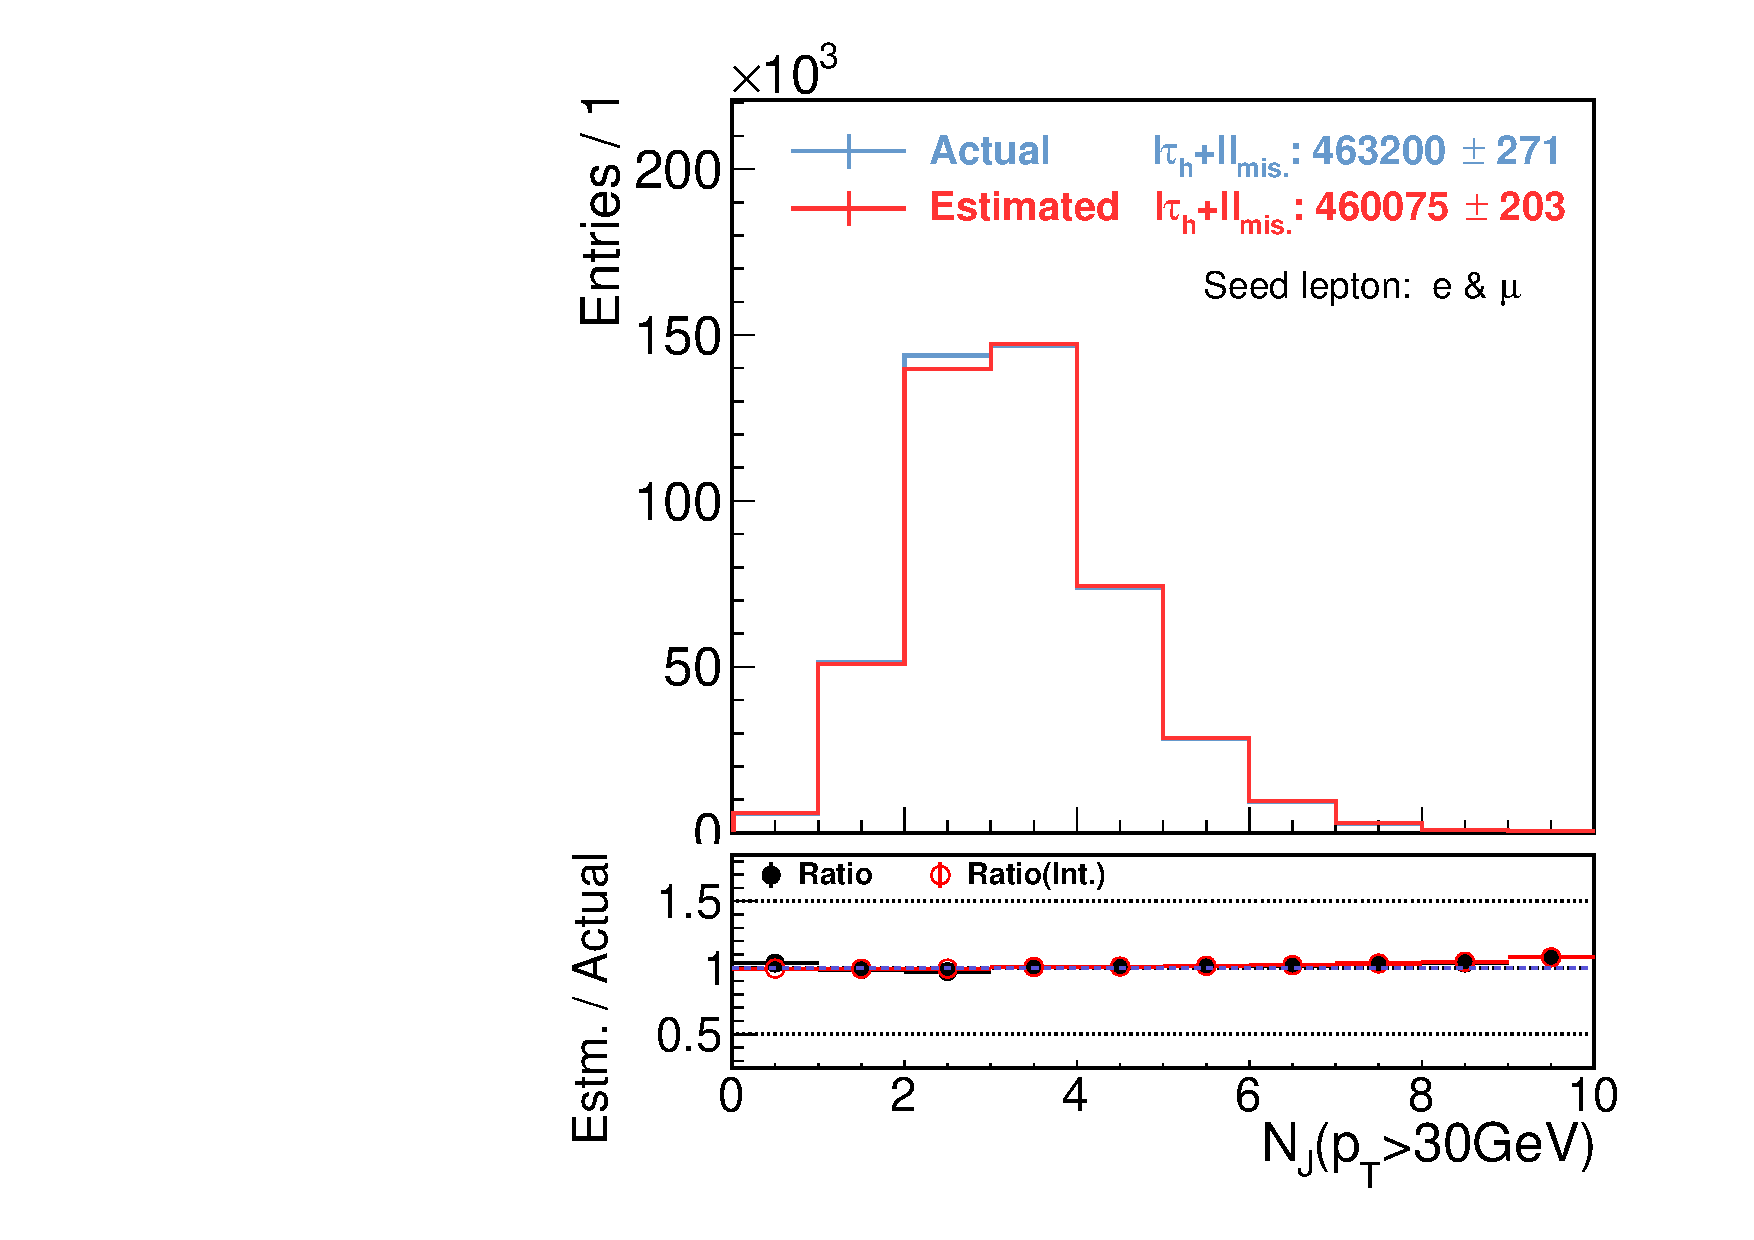
\includegraphics[width=0.32\textwidth]{figures/BGestimation/ObjReplacement/mcClosure/All_emu/All_emu_nJet30__trMode4_NoSys.pdf}}
    \subfigure[]{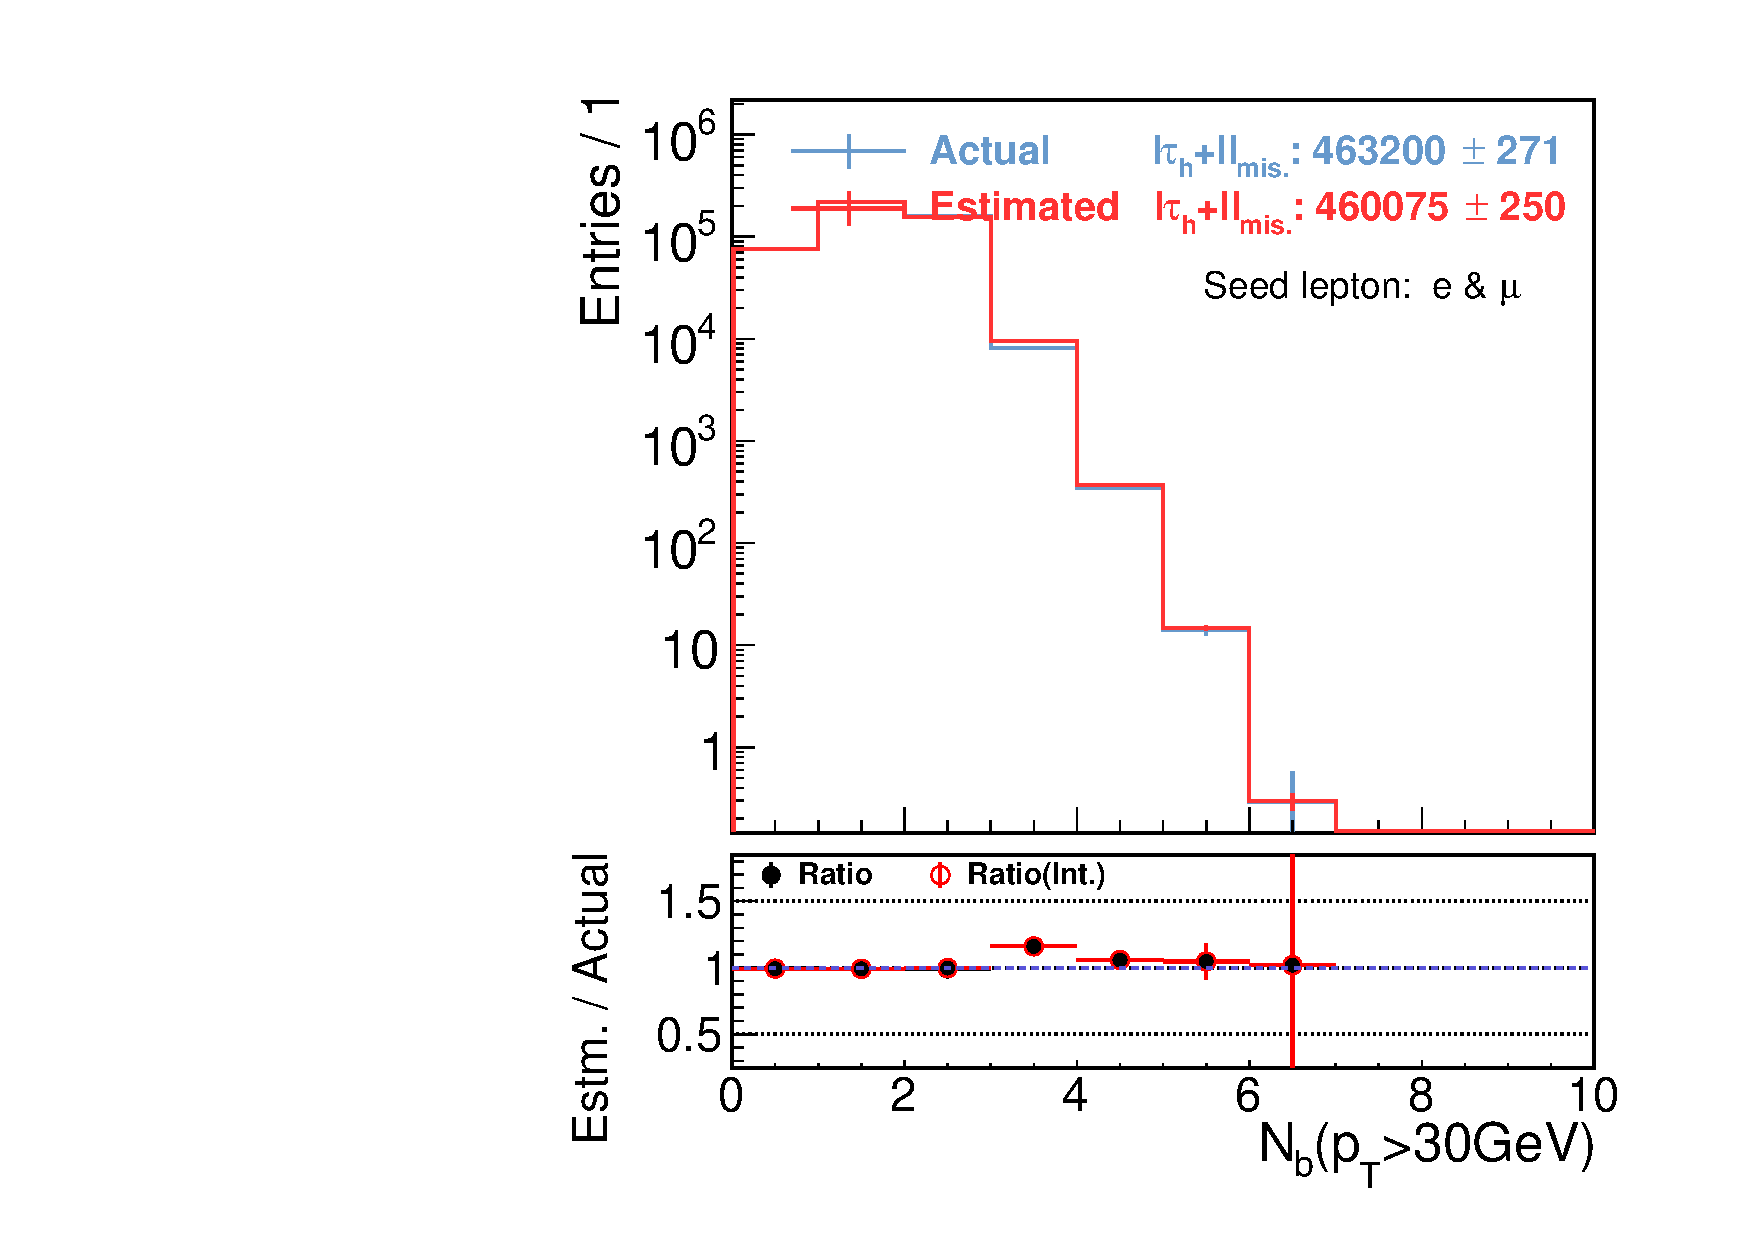
\includegraphics[width=0.32\textwidth]{figures/BGestimation/ObjReplacement/mcClosure/All_emu/All_emu_nBJet30__trMode4_NoSys.pdf}}
    \caption{ MC closure test for \textbf{combined estimation of missing lepton rep. and tau rep.} using $t\bar{t}$ MC sample. Seed events are collected by the single-lepton trigger. $p_T>35\gev$ for the leading lepton is required. \textbf{Both electrons and muons in the seed events are replaced}. Red points in the bottom plots show the ratio of integrated yields for the two histograms above the x-position that the point indicates. \label{fig::ObjReplace::mcClosure_All_emu} }
\end{figure}
 %%%%%%%%%%%%%%%%%%%%%%%%%%
